\documentclass[fleqn,11pt]{article}

	\usepackage[letterpaper,margin=0.75in]{geometry}
	
	\usepackage{amsmath}
	\usepackage{booktabs}
	\usepackage{graphicx}
	\usepackage{listings}
	
	\setlength{\parindent}{1.4em}
	
	\begin{document}
	
	\lstset{
	  language=Python,
	  basicstyle=\small,          % print whole listing small
	  keywordstyle=\bfseries,
	  identifierstyle=,           % nothing happens
	  commentstyle=,              % white comments
	  stringstyle=\ttfamily,      % typewriter type for strings
	  showstringspaces=false,     % no special string spaces
	  numbers=left,
	  numberstyle=\tiny,
	  numbersep=5pt,
	  frame=tb,
	}
	
	\title{TCP Congestion Control}
	
	\author{Chris Johnson}
	
	\date{19 March 2018}
	
	\maketitle
	
	\section{Test 1}
	
	The first test run was just a simple file transfer on a basic, one-hop network.
	After integrating TCP Tahoe congestion control into the TCP implementation,
	a large pdf file was transferred with no loss on a 10Mbps link with a 100ms propagation delay.
	During this test, every change in the size of the congestion window was logged
	with the simulation time and the size of the window. The maximum segment size was set
	to 1,000 bytes, and the initial slow start threshold was set to 100,000 bytes.

	\subsection{Results}
	
	{
		\centering
		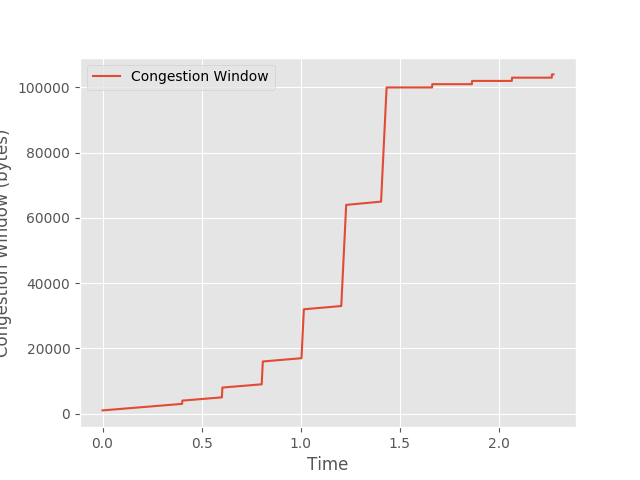
\includegraphics[]{cwnd1}
		
	}
	
	\subsection{Analysis}
	
	This test and the data produced show the effect slow start has on the growth rate
	of the congestion window size. The distinction between exponential and additive increase
	noticeable. Just before 1.5 seconds into the simulation, the congestion window size reaches
	the threshold, and additive increase begins. Before 1.5 seconds, the growth was clearly
	exponential. Once the threshold is reached, additive increase causes a more gradual linear
	growth. The steps in the graph are due to the latency on the link. With a 100ms propagation
	delay, the round trip time is 200ms. This means the first packet sent out from the window
	will be acknowledged 200ms later, while the rest of the ACKs for packets in that same window
	are received in quick succession after the first. The jumps indicate each packet from one window
	being acknowledged rapidly, and the size of the window is shown to double each "cycle" until the
	threshold is reached.
	
	\section{Test 2}
	
	After a simple test with no loss, the file transfer was repeated, however, this time,
	sequence number 14,000 was dropped. After this loss, no other loss event occurred. This
	test serves to illustrate the effect of packet loss on this implementation of TCP.
	
	
	\subsection{Results}
	
	{
		\centering
		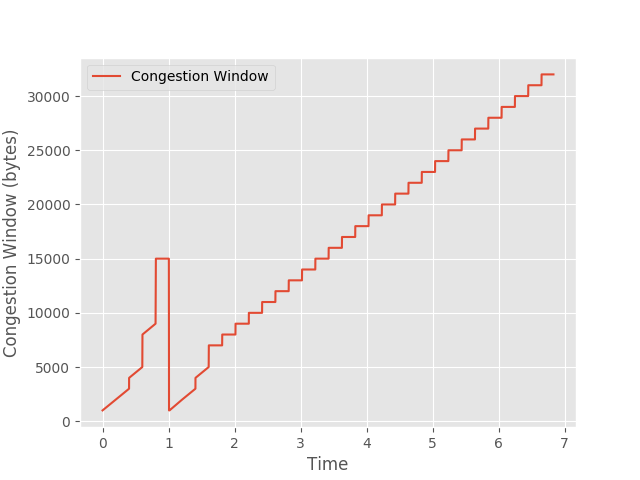
\includegraphics[]{cwnd2}
		
		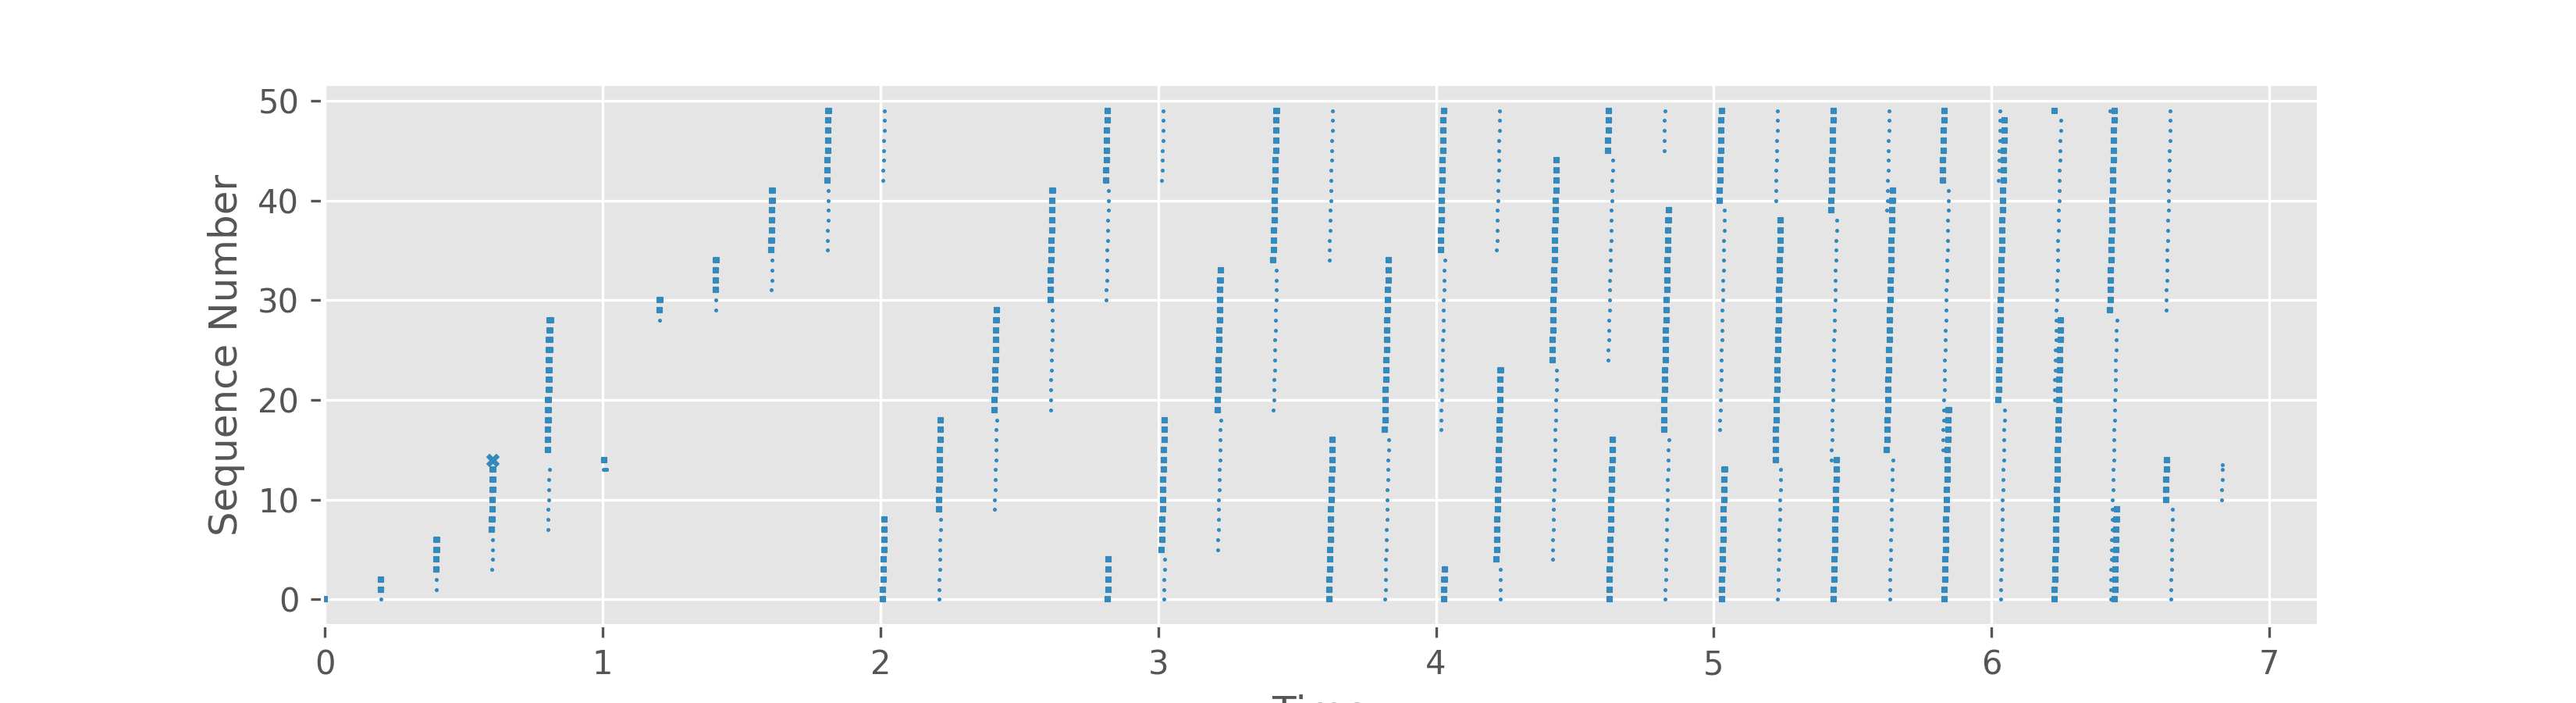
\includegraphics[width=17cm]{sequence2}
		
	}

	\subsection{Analysis}
	
	Just from the congestion window plot, it is evident that the loss of a single packet affects
	congestion window growth a great deal. Because this loss occurred during slow start, not only is
	the congestion window size reset, but the slow start threshold is set very low. During the second
	slow start period, this threshold is reached very quickly, and additive increase is started when
	the congestion window size is only 7,000 bytes. All of this has the effect of the congestion
	window never coming close to reaching the size it reached in the first test. Instead, the size
	of the congestion window at the end of the second test is about one third the size it was in
	the first test.
	
	The sequence plot appears as expected - the points grouped in lines reflecting the packets sent in
	one window. At the end of the third group, the packet is dropped. As the ACKs are received for that window, the next window begins transferring as well, until the third duplicate ACK is received. This
	triggers slow start again, and since only one packet was dropped, the ACK that is received while
	the window is still just 1,000 bytes acknowledges the next window as well, not just the dropped
	packet. So slow start continues from the next window, until additive increase takes over just before
	2 seconds into the simulation. From this point on, the window only grows by one MSS each time
	an entire window is acknowledged. This also matches the graph from Kevin Fall and Sally Floyd's
	graph on the same topic from their paper about SACK TCP. 
	
	\section{Test 3}
	
	The same configuration was used for the third test instead of a single loss, two packets were dropped.
	In addition to sequence 14,000, sequence 26,000 was also dropped in this test.
	
	\subsection{Results}
	
	{
		\centering
		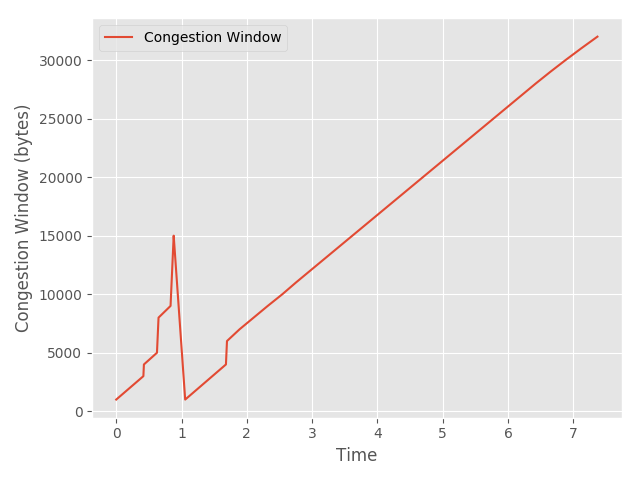
\includegraphics[]{cwnd3}
		
		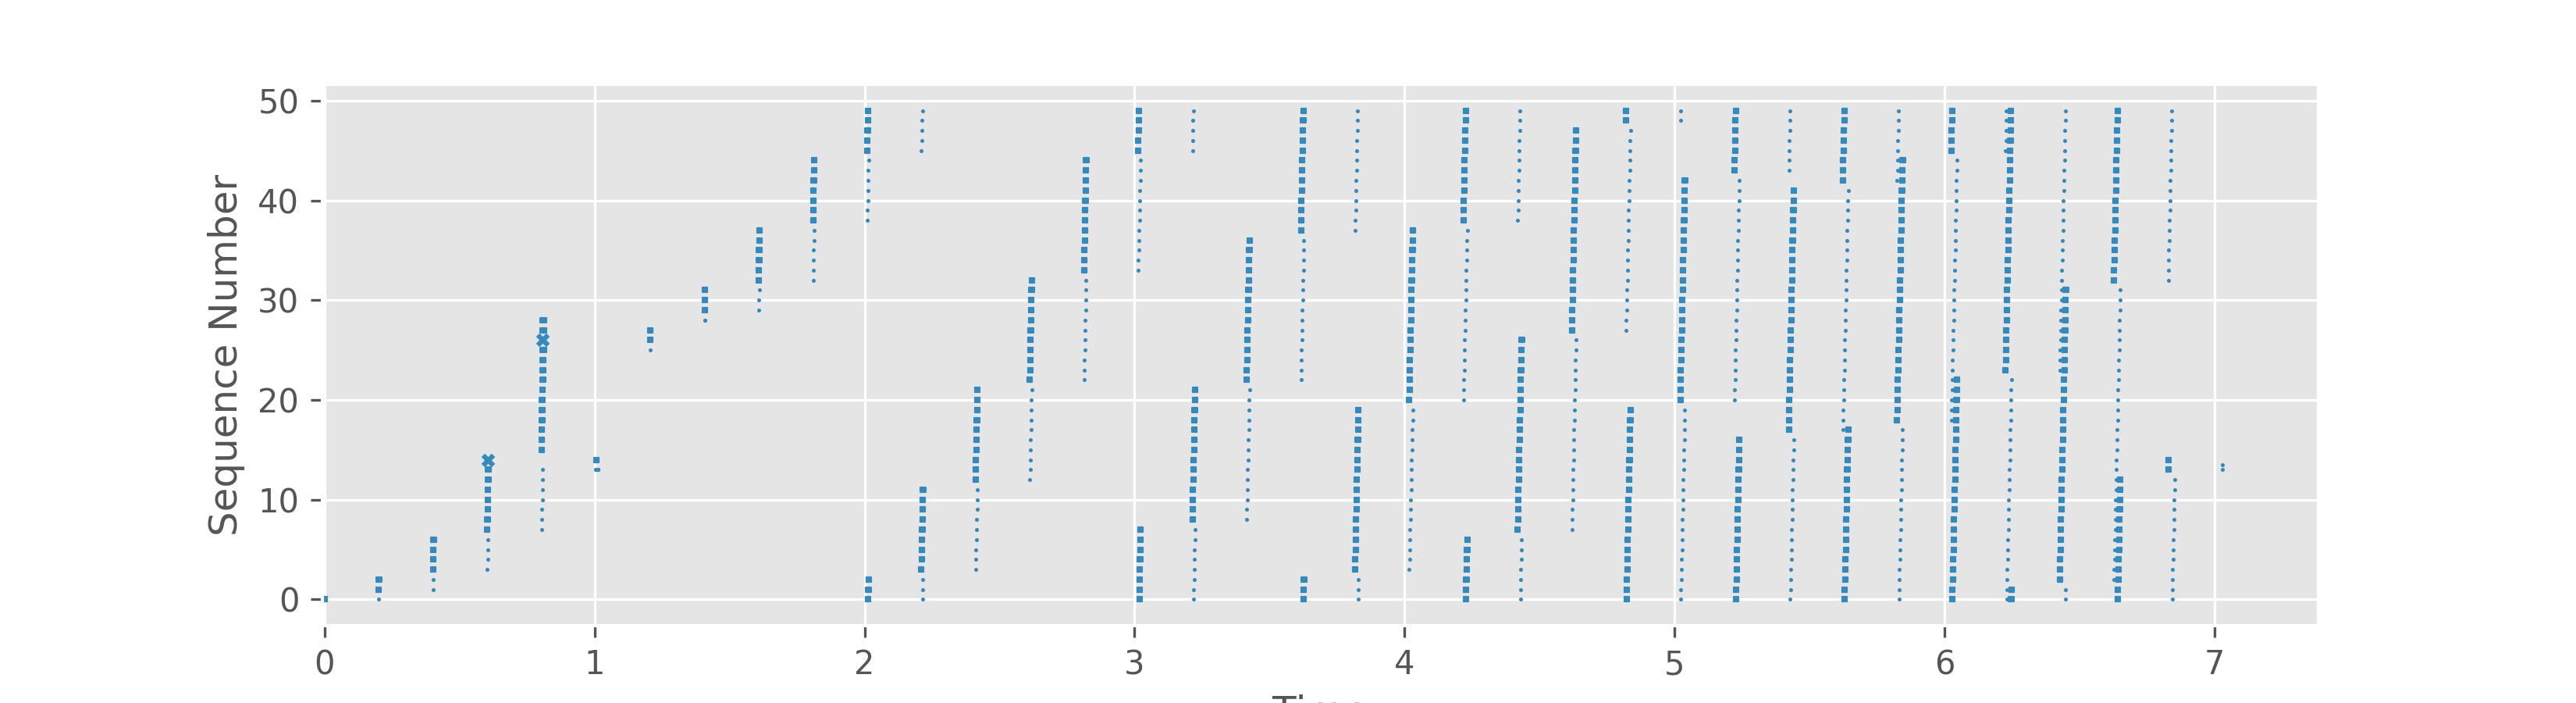
\includegraphics[width=17cm]{sequence3}
		
	}
	
	\subsection{Analysis}
	
	The results of the third test were very similar to the results from the previous test. Both
	the congestion window and sequence number plots resemble the plots generated from the second
	set of results. The reason for this is that the sender never "realized" that the second
	packet was dropped. Before retransmitting the 15th packet, the sender had already transmitted
	the next window. This window was larger than the window that the 15th packet was sent in. Sequence
	14,000 was sent as part of the fourth window, which was 8,000 bytes. The next window would have 
	reached 16,000 bytes, and it contained the 27th packet, which was also dropped. This means that
	the next loss occurred while the sender was waiting for the first dropped packet to be
	acknowledged. When the sender retransmitted, it did not keep track of the rest of the outstanding
	packets, and they would have been retransmitted as well. The receiver, however, acknowledged
	all outstanding packets up to the 27th packet, so the sender resumed slow start by sending the
	27th packet as the first packet of the second window in the second round of slow start.
	The only difference between the second test and this test was that in the second test, after
	slow start was restarted, the second window began with sequence 29,000 as opposed to sequence
	26,000.
	
	Overall, this change had little effect on the file transfer. Where the last packet was sent
	in the second test at around 7 seconds, the last packet of test 3 was sent at around 7.2 seconds.
	In the second test, additive increase began at about 1.9 seconds. In the third test, it began at
	roughly 2.1 seconds. Besides a slight variation in both plots, the impact of the second dropped packet
	was much less than the impact of the first. It should be noted that this is largely due to the timing
	of the second loss. If the second packet was dropped later in the transfer, the window size
	would be reset again, and there would be a more noticeable delay from the second loss. Like
	test 2, the sequence plot matches the SACK TCP paper plot of the same scenario.
	
	\section{Test 4}
	
	The last test consisted of the same process, only dropping an additional packet during the file
	transfer. The same two packets as test 3 were dropped, as well as sequence number 28,000.
	
	\subsection{Results}
	{
		\centering
	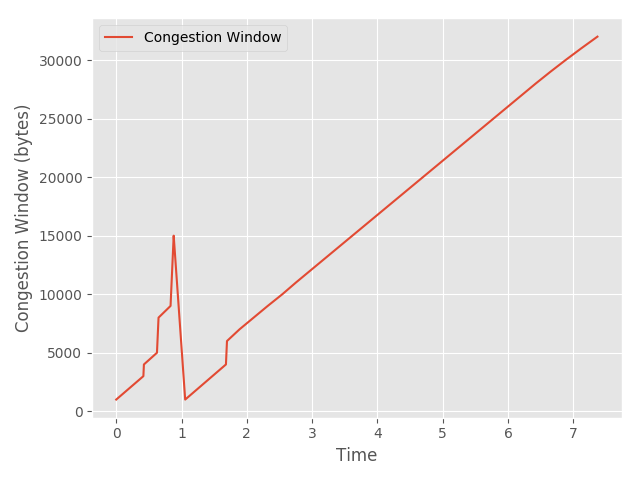
\includegraphics[]{cwnd4}
	
	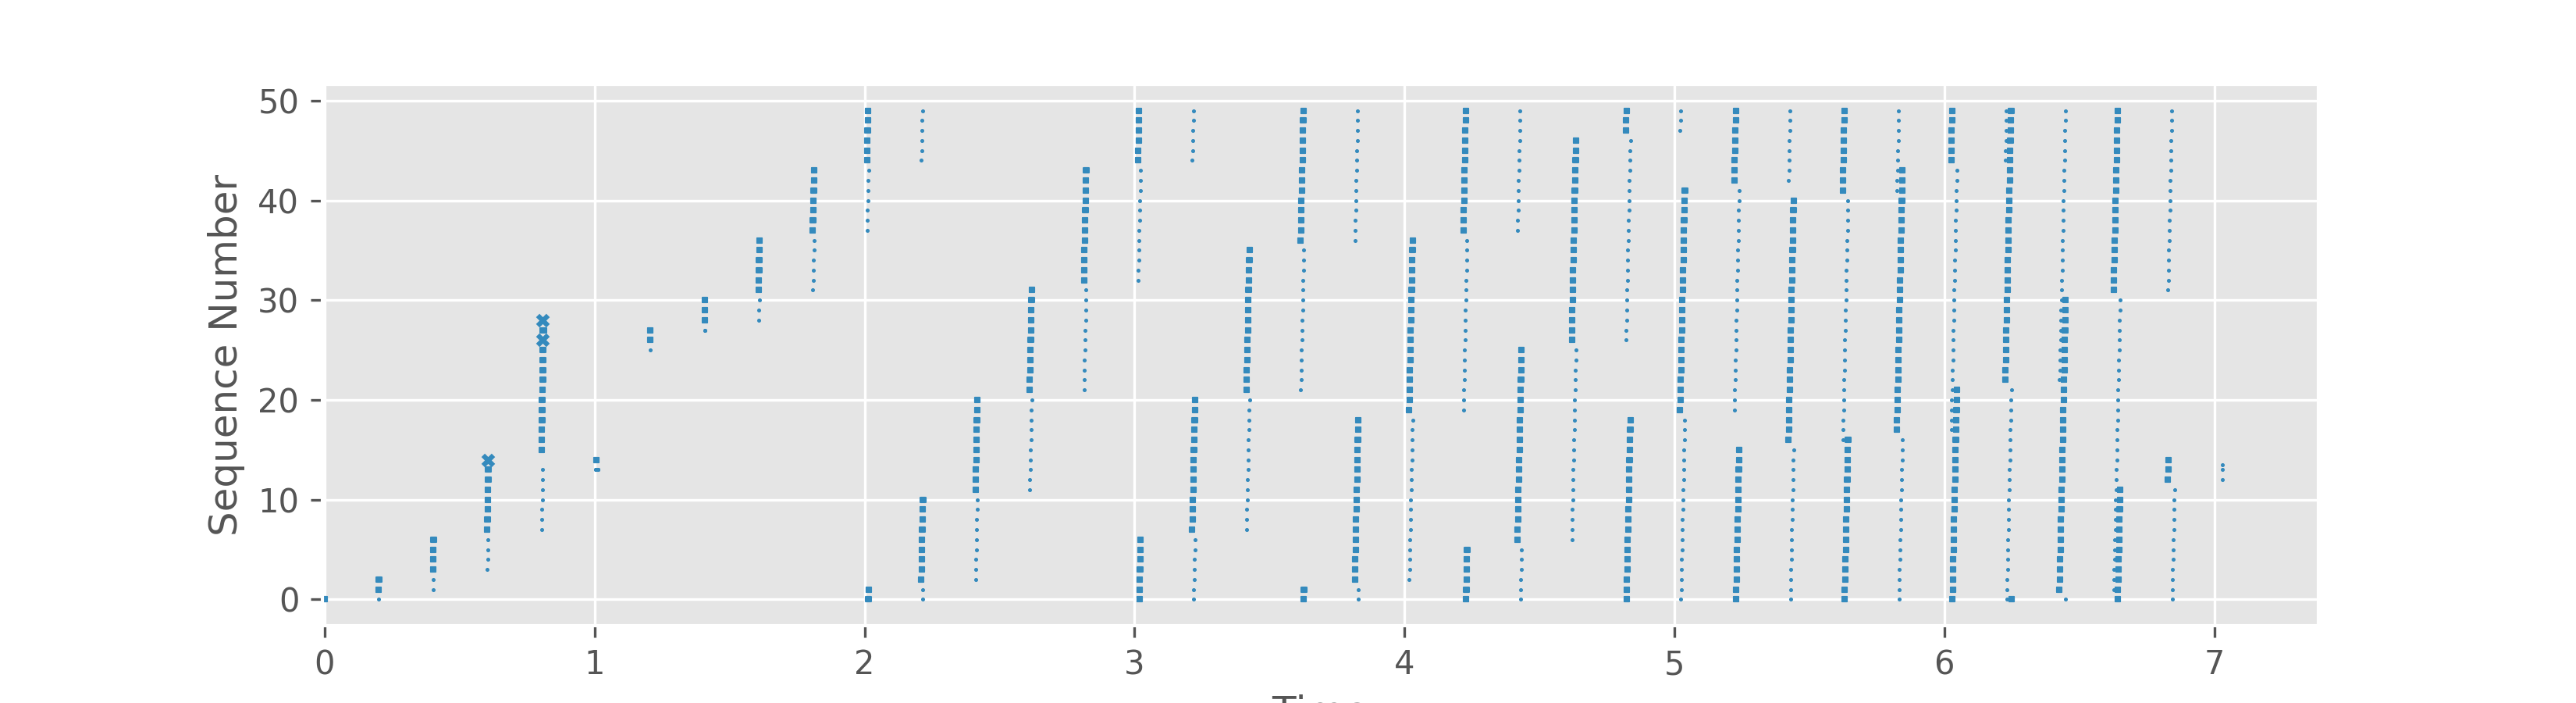
\includegraphics[width=17cm]{sequence4}
	
	}
	\subsection{Analysis}
	
	The congestion window plots of the third and fourth tests are identical. The sequence number
	plots are also nearly the same. The main difference between the sequence plots is that sequence
	28,000 had to be resent. During test 3, sequence 28,000 was acknowledged when sequence 26,000 was 
	retransmitted. In test 4, sequence 28,000 was lost, so it did have to be sent again. All this means
	is that the file transfer during test 4 was 1,000 bytes behind test 3. Other than that, the sequences are identical. As in the previous two tests, the graph used in the TCP SACK paper of TCP Tahoe with three packets dropped matches the graph generated from the fourth test. 
	
	\end{document}
	